\section{Image Analysis System}

\label{image_analysis_design}

The purpose of the image analysis application is to convert the raw input from the Kinect sensor into a detected
object, at which our turret may fire. To do this, it should receive image and depth data from the Kinect.
This will happen asynchronously, and therefore one frame of each image and depth must be matched to create a
"composite" frame, which should represent a view of the world at a specific point in time. This system must
also be able to handle a dropped frame from either part of the sensor, so that if one drops frames more
often than the other, the frames stay in sync. This can easily be done using the timestamps added to the data
by the Kinect.

The system must then run image analysis on the image data stored, and use the results combined with the depth
data to determine detected objects position in 3D space. Any detected object must then be matched with past
detected object, to see if it is reasonably the same object. If it is, the existing object should be updated,
if not, a new object should be saved.

Finally the system should check if any objects are suitable for targeting, for example by checking the amount of
data available on the object. If any object is suitable, it should be encoded and send to the NXT.
This can be visualized with the flowchart seen in \autoref{fig:nxtkinectflow} .

\begin{figure}[hbtp]
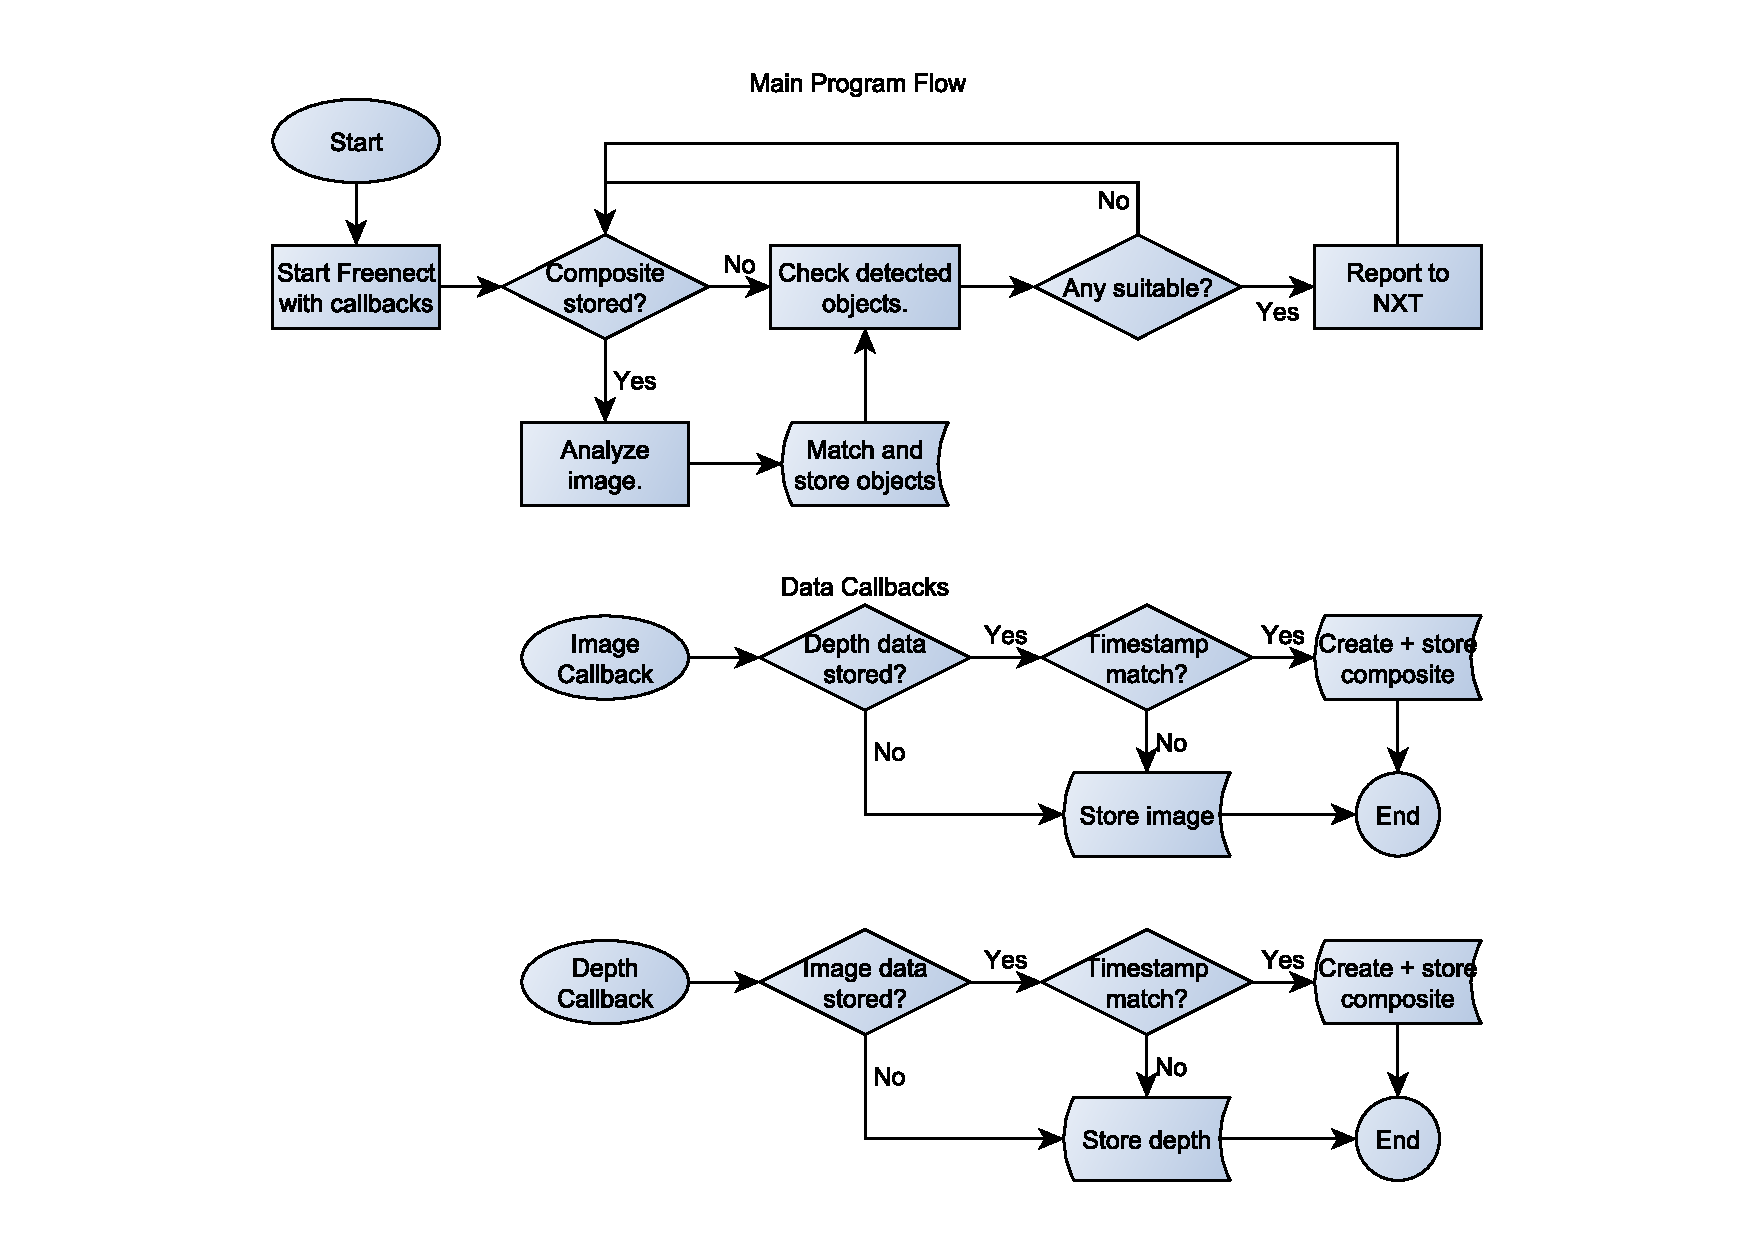
\includegraphics[width=0.90\textwidth]{img/nxtkinectflow.pdf}
\caption{Flowchart} 
\label{fig:nxtkinectflow} 
\end{figure}

As the system is written in Python, it should be divided into several modules containing classes
and functions related to that module. The necessary modules for this system are:
\begin{itemize}
  \item{Analyzer}\\
  Contains the central Analyzer class which is used for fetching and comparing data, and storing (or discarding) it
  correctly.
  \item{Coordinate}\\
  Contains classes for representing points in space, functionality for converting these, and doing simple calculations
  using these points.
  \item{Objects}
  Contains classes for storing detected objects, with all necessary information. Also intermediate data needed to
  detect objects.
  \item{USB Com}
  Contains classes for managing the USB connection to the NXT, and formatting the data to be send, so it complies with
  our protocol.
\end{itemize}

This leads to the module diagram seen in \autoref{fig:nxtkinect1}.

\begin{figure}[hbtp]
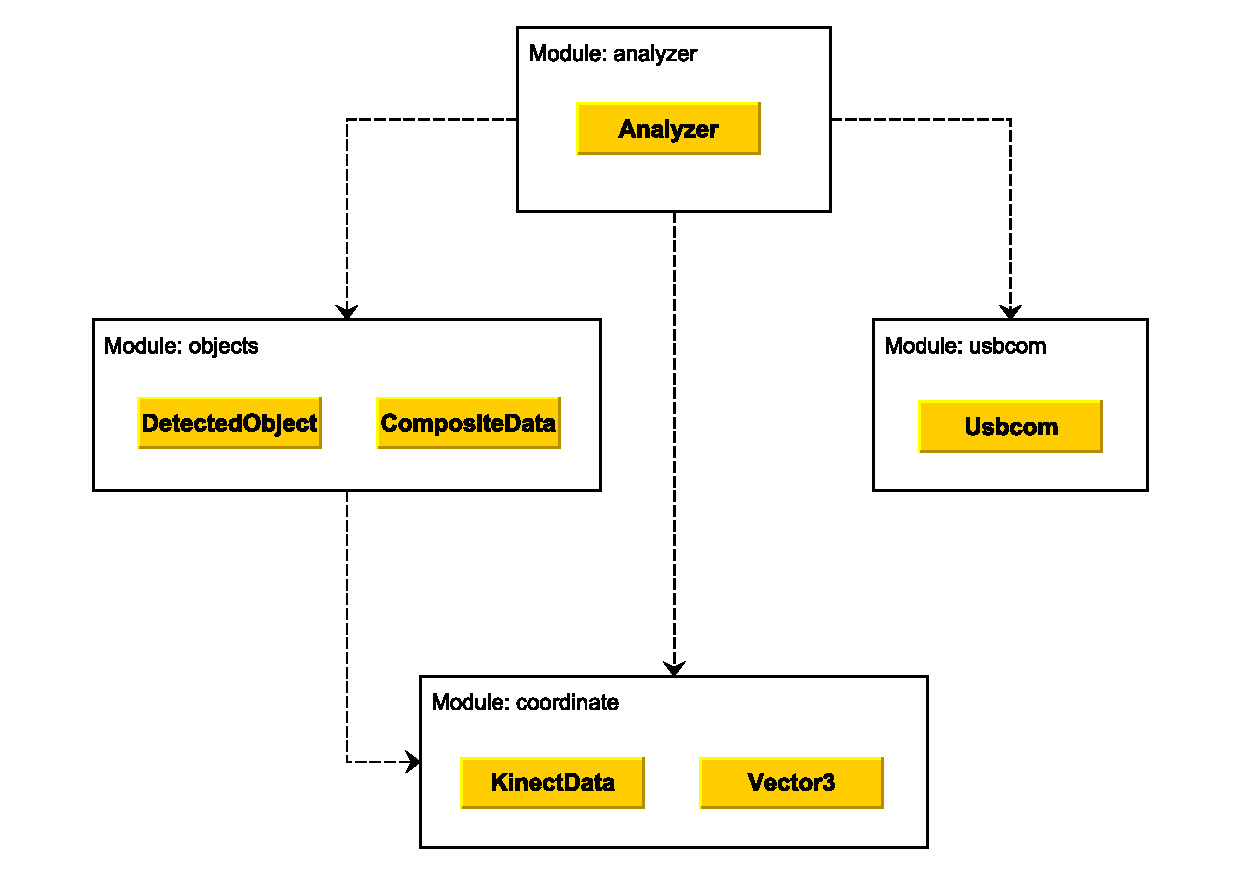
\includegraphics[width=0.90\textwidth]{img/nxtkinect1.pdf}
\caption{Module Diagram} 
\label{fig:nxtkinect1} 
\end{figure}

An explanation of the shown classes follows, starting from the bottom.
\begin{itemize}
  \item{KinectData}\\
  This is a \ac{pod} class, that stores a point in 3D space, as received from the Kinect. This means the horizontal
  and vertical images are stored as pixel-positions on the input image, and the depth is stored using a special scale
  implemented on the Kinect.
  \item{Vector3}\\
  This class also stores a point in 3D space, though it does so in an arguably more useful coordinate system. 
  The zero-point of this system is the Kinect sensor, the z-axis is the line from the Kinect to whatever it is pointed
  at, the y-axis is vertical and the x-axis is horizontal, perpendicular to the direction the Kinect points.
  This coordinate system will be using a scale of millimeters. The Vector3 class will also contain methods to
  convert a KinectData point to Vector3 point, and will implement necessary vector arithmetic.
  \\
  \item{CompositeData}\\
  This is another \ac{pod} class, that contains one frame of image data, and one frame of depth data,
  as paired by the analyzer. This data will be stored in the format which it can most efficiently be passed
  to \ac{opencv}, which is a special array implementation, using a python library called NumPy\cite{numpy}.
  \item{DetectedObject}\\
  This class stores information about a tracked and detected object. It contains a list of Vector3 instances,
  describing the position of the object for each frame in which it has been identified. Additionally, it has two
  timestamps, one for when the object was first detected, and one for when the last update to the object took place.
  The class will have functionality to determine the object's velocity and direction, as well as to determine if there
  is a suitable amount of information to predict the object's path.
  \\
  \item{Usbcom}\\
  This class handles the connection to the NXT. It will contain a handle to a USB Connection, and have functionality
  to encode data, as well as send and receive data to and from the NXT.
  \\
  \item{Analyzer}\\
  This is the class that ties the other classes together. It will contain a list of DetectedObjects,
  a list of CompositeData to be analyzed and an instance of the Usbcom class for communication.
  The responsibilities of this class will be the following: Match a received
  image frame to the correct depth frame as these will be received asynchronously, invoke the \ac{opencv} functions
  to run image analysis, and finally, to pass suitable objects to the usb class for transfer.
\end{itemize}

With this we end up with the class diagram seen in \autoref{fig:nxtkinect2}. This diagram shows the interfaces
of each class, but leaves out any functionality used only for internal calculations, as these are left up to 
the implementation.

\begin{figure}[hbtp]
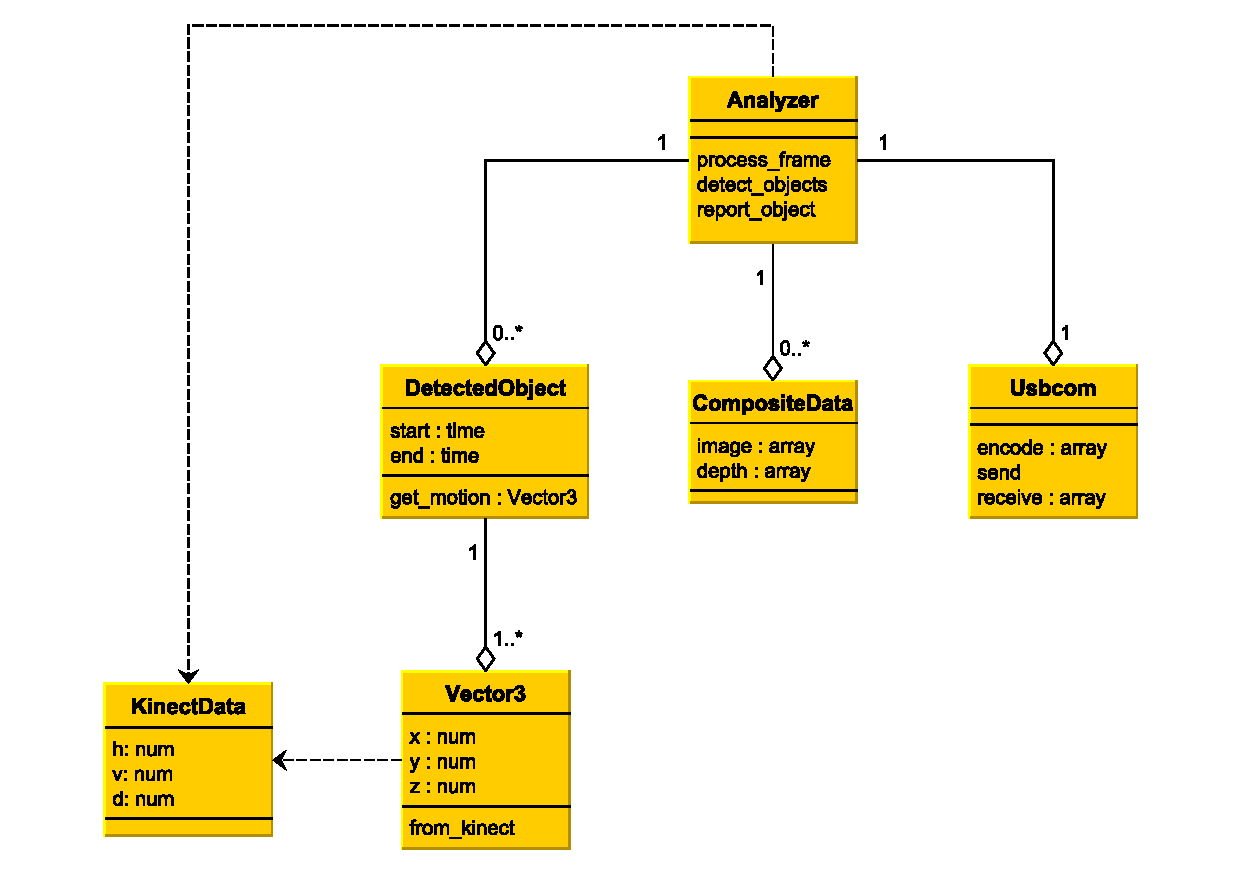
\includegraphics[width=0.90\textwidth]{img/nxtkinect2.pdf}
\caption{Class Diagram} 
\label{fig:nxtkinect2} 
\end{figure}

